\documentclass[11pt]{charter}

% El títulos de la memoria, se usa en la carátula y se puede usar el cualquier lugar del documento con el comando \ttitle
\titulo{Sensor inteligente} 

% Nombre del posgrado, se usa en la carátula y se puede usar el cualquier lugar del documento con el comando \degreename
\posgrado{Carrera de Especialización en Sistemas Embebidos} 
%\posgrado{Carrera de Especialización en Internet de las Cosas} 
%\posgrado{Carrera de Especialización en Intelegencia Artificial}
%\posgrado{Maestría en Sistemas Embebidos} 
%\posgrado{Maestría en Internet de las cosas}

% Tu nombre, se puede usar el cualquier lugar del documento con el comando \authorname
\autor{Martín Alejandro Mello Teggia} 

% El nombre del director y co-director, se puede usar el cualquier lugar del documento con el comando \supname y \cosupname y \pertesupname y \pertecosupname
\director{Pablo Castillo}
\pertenenciaDirector{CoNEA} 
% FIXME:NO IMPLEMENTADO EL CODIRECTOR ni su pertenencia
\codirector{} % si queda vacio no se deberíá incluir 
\pertenenciaCoDirector{}

% Nombre del cliente, quien va a aprobar los resultados del proyecto, se puede usar con el comando \clientename y \empclientename
\cliente{Cristian Muzzio}
\empresaCliente{HiTec S.R.L.}

% Nombre y pertenencia de los jurados, se pueden usar el cualquier lugar del documento con el comando \jurunoname, \jurdosname y \jurtresname y \perteunoname, \pertedosname y \pertetresname.
\juradoUno{Nombre y Apellido (1)}
\pertenenciaJurUno{pertenencia (1)} 
\juradoDos{Nombre y Apellido (2)}
\pertenenciaJurDos{pertenencia (2)}
\juradoTres{Nombre y Apellido (3)}
\pertenenciaJurTres{pertenencia (3)}
 
\fechaINICIO{23 de octubre de 2020}		%Fecha de inicio de la cursada de GdP \fechaInicioName
\fechaFINALPlanificacion{11 de diciembre de 2020} 	%Fecha de final de cursada de GdP
\fechaFINALTrabajo{22 de agosto de 2021}		%Fecha de defensa pública del trabajo final


\begin{document}

\maketitle
\thispagestyle{empty}
\pagebreak


\thispagestyle{empty}
{\setlength{\parskip}{0pt}
\tableofcontents{}
}
\pagebreak


\section{Registros de cambios}
\label{sec:registro}


\begin{table}[ht]
\label{tab:registro}
\centering
\begin{tabularx}{\linewidth}{@{}|c|X|c|@{}}
\hline
\rowcolor[HTML]{C0C0C0} 
Revisión & \multicolumn{1}{c|}{\cellcolor[HTML]{C0C0C0}Detalles de los cambios realizados} & Fecha      \\ \hline
0.1      & Creación del documento                                          & 23/10/2020 \\ \hline
0.2      & Avances hasta punto 6 inclusive (sin user stories)                                         & 06/11/2020 \\ \hline
\end{tabularx}
\end{table}

\pagebreak



\section{Acta de constitución del proyecto}
\label{sec:acta}

\begin{flushright}
Buenos Aires, \fechaInicioName
\end{flushright}

\vspace{2cm}

Por medio de la presente se acuerda con el Ing. \authorname\hspace{1px} que su Trabajo Final de la \degreename\hspace{1px} se titulará ``\ttitle'', consistirá esencialmente en el prototipo preliminar de un sistema de control de temperatura de un calefón, y tendrá un presupuesto preliminar estimado de 600 hs de trabajo y \textcolor{red}{\$XXX}, con fecha de inicio \fechaInicioName\hspace{1px} y fecha de presentación pública \fechaFinalName.

Se adjunta a esta acta la planificación inicial.

\vfill

% Esta parte se construye sola con la información que hayan cargado en el preámbulo del documento y no debe modificarla
\begin{table}[ht]
\centering
\begin{tabular}{ccc}
\begin{tabular}[c]{@{}c@{}}Ariel Lutenberg \\ Director posgrado FIUBA\end{tabular} & \hspace{2cm} & \begin{tabular}[c]{@{}c@{}}\clientename \\ \empclientename \end{tabular} \vspace{2.5cm} \\ 
\multicolumn{3}{c}{\begin{tabular}[c]{@{}c@{}} \supname \\ Director del Trabajo Final\end{tabular}} \vspace{2.5cm} \\
%\begin{tabular}[c]{@{}c@{}}\jurunoname \\ Jurado del Trabajo Final\end{tabular}     &  & \begin{tabular}[c]{@{}c@{}}\jurdosname\\ Jurado del Trabajo Final\end{tabular}  \vspace{2.5cm}  \\
%\multicolumn{3}{c}{\begin{tabular}[c]{@{}c@{}} \jurtresname\\ Jurado del Trabajo Final\end{tabular}} \vspace{.5cm}                                                                     
\end{tabular}
\end{table}



\newpage
\section{Descripción técnica-conceptual del proyecto a realizar}
\label{sec:descripcion}

\subsection*{Introducción general al tema}

El mantenimiento predictivo es indispensable en la industria farmacéutica, ya que la falla de un actuador puede implicar la pérdida de un lote completo de medicamentos, procesos que pueden consumir días enteros, y valiosos insumos.

Existe bibliografía que permite evaluar el desgaste de un motor mediante el análisis de sus vibraciones, procesando la información adquirida en el dominio de la frecuencia, y datos estadísticos en el dominio del tiempo.

En la empresa Hitec S.R.L. se desarrolló un sistema para realizar esta tarea, pero el objetivo del presente trabajo es trasladar el procesamiento al edge (MCU del sensor), permitiendo extraer información de los sensores y no solo datos de mediciones.

Este producto se presenta como un sensor innovador, ya que las mediciones para mantenimiento predictivo se realizan mayormente offline. La integración de este sensor permite integrar el mantenimiento en la nube, lo que lo diferencia de la mayor parte de la competencia.

\subsection*{Descripción del producto a desarrollar}

El objetivo del hardware a desarrollar es adquirir y procesar datos de vibración y temperatura en el mismo sensor, para entregar información pre-procesada a una unidad central.

Para esto, el sensor deberá contar con un microcontrolador que realice las adquisiciones, procesamiento y comunicación de resultados, un circuito integrado que permita adquirir valores de vibración en tiempo real, un sensor de temperatura para medir las variaciones del dispositivo bajo análisis, y una memoria para almacenar datos de fabricación (y eventualmente calibración) independientes de la programación del microcontrolador. 

En la figura \ref{fig:diagramaBloques} se presenta un diagrama en bloques del sistema, donde puede verse las relaciones previamente mencionadas.

\begin{figure}[htpb]
\centering 
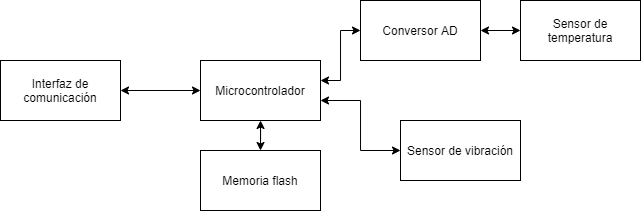
\includegraphics[width=1\textwidth]{./Figuras/diagramaBloques.png}
\caption{Diagrama en bloques del sistema}
\label{fig:diagramaBloques}
\end{figure}

El integrado de vibración debe ser encuestado a frecuencia constante, para garantizar el espaciamiento temporal de los valores medidos. El sensor de temperatura será encuestado solo para valores estadísticos, por lo que no será necesario un retardo estable entre mediciones.

El microcontrolador debe poder adquirir los valores, computar parámetros estadísticos, procesar el paso al dominio de la frecuencia, y extraer también información de esta representación. Es importante que el distanciamiento de muestras en el dominio del tiempo sea constante, para evitar el jitter en frecuencia. Finalmente, deberá almacenar los resultados obtenidos, e informarlos con una frecuencia configurable a un dispositivo central.

El sensor estará diseñado para soportar descargas electrostáticas, y otros eventos de compatibilidad electromagnética que puedan surgir en la industria. Para esto, se buscará cumplir con las siguientes normas:
\begin{itemize}
\item IEC 61000-4-2: ESD
\item IEC 61000-4-4: EFT
\item IEC 61000-4-5: Surge
\end{itemize}

De ser posible, también es de interés que el sensor sea ATEX, para poder operar en entornos que requieren que los dispositivos sean anti-explosivos.



%\begin{consigna}{red}
%El objetivo es que el lector en una o dos páginas entienda de qué se trata el proyecto y cuáles son sus desafíos, su motivación y su importancia.
%Se debe destacar claramente cuál es el valor que agrega el proyecto a realizar. ``El presente proyecto se destaca especialmente por incorporar tal cosa... Esto lo diferencia de otros sistemas similares en que ...''
%
%Puede ser útil incluir en esta sección la respuesta a alguna de estas preguntas:
%
%\begin{itemize}
%\item ¿Cómo se vincula este proyecto con la misión de la organización?
%\item ¿Cómo se inserta este proyecto en el modelo de negocio de la organización?
%\item ¿Ayuda a la explicación si se incluye un lienzo Canvas del Modelo de Negocio?
%\item ¿En qué estado del ciclo de vida está el producto que se desea reemplazar o mejorar?
%\item ¿Cuales son las necesidades que debe satisfacer?
%\item ¿Por dónde pasa la innovación?
%\end{itemize}
%
%La descripción técnica-conceptual \textbf{debe incluir al menos un diagrama en bloques del sistema }y una frase como la siguiente: ``En la Figura \ref{fig:diagBloques} se presenta el diagrama en bloques del sistema. Se observa que...''. Luego recién más abajo de haber puesto esta frase se pone la figura. La regla es que las figuras nunca pueden ir antes de ser mencionadas en el texto, porque sino el lector no entiende por qué de pronto aparece una figura.
%
%\vspace{25px}
%
%\begin{figure}[htpb]
%\centering 
%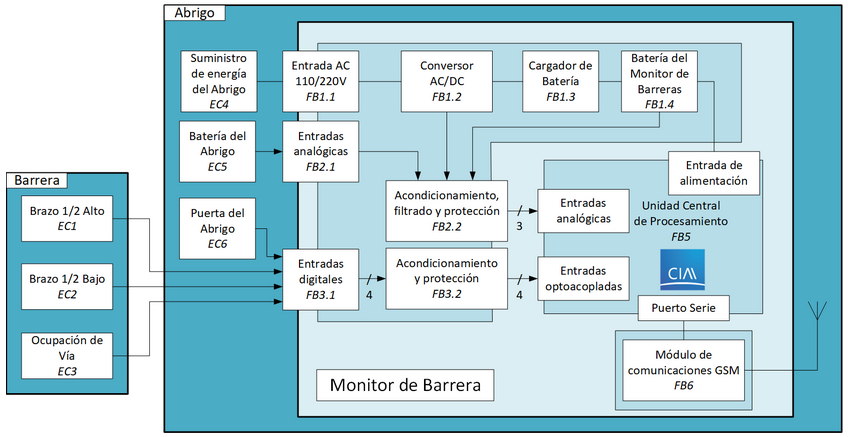
\includegraphics[width=.7\textwidth]{./Figuras/diagBloques.png}
%\caption{Diagrama en bloques del sistema}
%\label{fig:diagBloques}
%\end{figure}
%
%\vspace{25px}
%
%El tamaño de la tipografía en la figura debe ser adecuado para que NO pase lo que ocurre acá, donde el lector debe esforzarse para poder leer el texto. Los colores usados en el diagrama deben ser adecuados, tal que ayuden a comprender mejor el diagrama.
%\end{consigna}


\section{Identificación y análisis de los interesados}
\label{sec:interesados}

%\begin{consigna}{black}
%Nota: (borrar esto y todas las consignas en color rojo antes de entregar este documento).
% 
%Es inusual que una misma persona esté en más de un rol, incluso en proyectos chicos.
% 
%Si se considera que una persona cumple dos o más roles, entonces sólo dejarla en el rol más importante. Por ejemplo:
%
%\begin{itemize}
%\item Si una persona es Cliente pero también colabora u orienta, dejarla solo como Cliente.
%\item Si una persona es el Responsable, no debe ser colocado también como Miembro del equipo.
%\end{itemize}
%
%Pero en cambio sí es usual que el Cliente y el Auspiciante sean el mismo, por ejemplo.

\begin{table}[ht]
%\caption{Identificación de los interesados}
%\label{tab:interesados}
\begin{tabularx}{\linewidth}{@{}|l|X|X|l|@{}}
\hline
\rowcolor[HTML]{C0C0C0} 
Rol           & Nombre y Apellido & Organización 	& Puesto 	\\ \hline
Auspiciante   &      Matías Montero             &       HiTec S.R.L.       	&      Contador  	\\ \hline
Cliente       & \clientename      &\empclientename	& Gerente I+D     	\\ \hline
Impulsor      & \clientename      &\empclientename	& Gerente I+D     	\\ \hline
Responsable   & \authorname       & FIUBA        	& Alumno 	\\ \hline
Colaboradores & Nicolás Dini & HiTec S.R.L. & Programador Senior \\ \newline 
			&	Luciano Gurevich  &    HiTec S.R.L.        	&  Data Scientist      	\\ \hline
Orientador    & \supname	      & \pertesupname 	& Director	Trabajo final \\ \hline
%Equipo        & - & - & -	\\ \hline
%Opositores    &           -        &       -       	&      -  	\\ \hline
Usuario final &       Martín Tomé            &  HiTec S.R.L.           	&  Jefe Servicio Técnico      	\\ \hline
\end{tabularx}
\end{table}


\begin{itemize}
\item Impulsor: \clientename tiene un conocimiento profundo de la industria, y las necesidades reales del producto.
\item Usuario Final: Martín Tomé tiene mucha experiencia con instalaciones, y puede ayudar a hacer más fácil de instalar y mantener el dispositivo, pero tiene poco tiempo disponible.
\item Colaborador: Nicolás Dini se ocupa de la interfaz de datos con la nube, el sensor tiene que poder finalmente comunicarse con su software.
\end{itemize}

%\end{consigna}



\section{1. Propósito del proyecto}
\label{sec:proposito}

El propósito de este proyecto es desarrollar un sensor inteligente, capaz de adquirir y pre-procesar datos de un sensor de vibración, para poder utilizarlos para realizar mantenimiento predictivo sobre motores de la industria farmacéutica.

\section{2. Alcance del proyecto}
\label{sec:alcance}

%\begin{consigna}{red}
%¿Qué se incluye y que no se incluye en este proyecto?
%
%Se refiere al trabajo a hacer para entregar el producto o resultado especificado. 
%
%Explicitar todo lo quede comprendido dentro del alcance del proyecto.
%
%Explicitar además todo lo que no quede incluido (``El presente proyecto no incluye...'')
%
%\end{consigna}

El presente proyecto incluirá el desarrollo completo del hardware del sensor, e incluirá el desarrollo del firmware para la realización de las siguientes funciones:

\begin{itemize}
\item Adquisición de valores de aceleración en 3 ejes.
\item Procesamiento de parámetros estadísticos en el dominio del tiempo.
	\begin{itemize}
	\item Valores de aceleración RMS (sin continua).
	\item Valores de aceleración continua.
	\item Factor de cresta.
	\end{itemize}
\item Procesamiento de los valores en frecuencia.
\item Configuración del ancho de banda deseado en frecuencia.
\item Implementación de un código de tramas para comunicación con la unidad central.
\item Adquisición de valores de temperatura para análisis estadístico
\item Compatibilidad con el producto teBox (HiTec S.R.L.)
\end{itemize}

El firmware no incluirá la posibilidad de modificar la cantidad de muestras analizadas en frecuencia, ni la orientación de los ejes en función de la posición de instalación del sensor.

\section{3. Supuestos del proyecto}
\label{sec:supuestos}

Para el desarrollo del presente proyecto se supone que:

\begin{itemize}
\item La empresa HiTec se ocupará de la compra del material necesario para la fabricación del sensor, así como también de todos aquellos elementos requeridos para realizar las pruebas iniciales del producto.
\item Se dispondrá de las unidades necesarias del producto teBox para pruebas de compatibilidad, y que el mismo cumple con sus especificaciones.
\item Se podrá consultar a Martín Tomé por cuestiones relacionadas a la instalación del sensor, a fin de desarrollar un dispositivo sencillo de utilizar desde su primera versión.
\item El laboratorio de pruebas de la empresa HiTec S.R.L. estará disponible durante toda la realización del proyecto, para realizar las pruebas necesarias con el instrumental presente en el mismo.
\item El protocolo que se defina para comunicar al sensor será estandar, o contará con amplia documentación para su implementación en el microcontrolador.
\item Los componentes utilizados podrán ser adquiridos en Argentina, o traídos del exterior, durante la duración del proyecto.
\item Se podrán realizar las pruebas de compatibilidad electromagnética en el país durante la realización del proyecto.
\end{itemize}


\section{4. Requerimientos}
\label{sec:requerimientos}

\begin{enumerate}
\item Requerimientos de construcción del equipo
	\begin{enumerate}
	\item El gabinete deberá poder acoplarse a un motor sin necesidad de modificar al mismo para hacerlo.
	\item Se debe proveer con el mecanismo de acople una forma de medir la temperatura del motor.
	\item El gabinete será metálico (prioridad menor).
	\end{enumerate}
\item Requerimientos de conexionado
	\begin{enumerate}
	\item Linea de alimentación que contenga 5 V y permita extraer una corriente máxima de 200 mA.
	\item Linea de datos referido al mismo punto que la alimentación
	\item Cables que provean la alimentación y datos con polaridad.
	\item Unificar en un único cable (prioridad menor)
	\end{enumerate}
\item Requerimientos asociados a la interfaz de comunicación
	\begin{enumerate}
	\item El sensor deberá poder comunicarse con el protocolo fijado por el producto teBox.
	\item El esquéma de comunicación será maestro esclavo, con el sensor recibiendo ordenes y ejecutando acciones en base a ellas.
	\item El sensor deberá poder reprogramarse a través de la misma interfaz de datos (prioridad menor)
	\end{enumerate}
\item Requerimientos asociados a la medición
	\begin{enumerate}
	\item El sensor deberá poder adquirir valores de aceleración en 3 ejes ortogonales entre si.
	\item El sensor deberá poder adquirir valores de temperatura del motor medido.
	\item Deberán poder extraerse datos estadísticos en el dominio del tiempo.
	\item Deberán poder extraerse datos en el dominio de la frecuencia.
	\item El sensor deberá guardar en una memoria flash externa información sobre máximos históricos, para evaluación durante servicios que se le ejecuten.
	\item Se deberá garantizar el espaciamiento temporal de los datos, para evitar jitter.
	\end{enumerate}
\item Requerimientos de validación
	\begin{enumerate}
	\item Cumplimiento norma IEC 61000-4-2: ESD.
	\item Cumplimiento norma IEC 61000-4-4: EFT.
	\item Cumplimiento norma IEC 61000-4-5: Surge.
	\end{enumerate}
\item Requerimientos de documentación
	\begin{enumerate}
	\item El código utilizará comentarios compatibles con Doxygen.
	\item Se proveerá un diagrama en bloques del procesamiento del microcontrolador.
	\item Se creará una entrada en la wiki de la empresa, con información de uso del firmware.
	\item Se generará un documento con el código de tramas para la comunicación de datos hacia y desde el microcontrolador.
	\end{enumerate}
\end{enumerate}


%\section{Historias de usuarios (\textit{Product backlog})}
%\label{sec:backlog}
%
%\begin{consigna}{red}
%Descripción: En esta sección se deben incluir las historias de usuarios y su ponderación (\textit{history points}). Recordar que las historias de usuarios son descripciones cortas y simples de una característica contada desde la perspectiva de la persona que desea la nueva capacidad, generalmente un usuario o cliente del sistema. La ponderación es un número entero que representa el tamaño de la historia comparada con otras historias de similar tipo.

\section{5. Entregables principales del proyecto}
\label{sec:entregables}

Los entregables principales del proyecto serán:
\begin{itemize}
\item Manual de uso
\item Diagrama esquemático
\item Código fuente
\item Diagrama de instalación
\item Certificados de compatibilidad electromagnética
\item Informe final

\end{itemize}


\section{6. Desglose del trabajo en tareas}
\label{sec:wbs}

\begin{enumerate}
\item Gestión del proyecto (88 hs)
	\begin{enumerate}
	\item Análisis de bibliografía existente y opciones desplegadas en el mercado (40 hs)
	\item Elaboración de la planificación del proyecto (40 hs)
	\item Definición de los casos de prueba (8 hs)
	\end{enumerate}
\item Diseño de hardware (104 hs)
	\begin{enumerate}
	\item Diseño de la arquitectura de hardware a utilizar (24 hs)
	\item Análisis y elección de un gabinete (16 hs)
	\item Diseño del PCB (40 hs)
	\item Elección de conectores (16 hs)
	\item Revisión del CAD del gabinete con el del PCB y los conectores (8 hs)
	\end{enumerate}
\item Desarrollo de firmware (232 hs)
	\begin{enumerate}
	\item Desarrollo de biblioteca para manejo de periféricos necesarios (16 hs)
	\item Desarrollo de biblioteca para adquisición y almacenamiento de valores de los sensores (40 hs)
	\item Procesamiento de valores para obtención de estadísticos (16 hs)
	\item Implementación de algoritmo de FFT (16 hs)
	\item Procesamiento de valores en el dominio de la frecuencia (40 hs)
	\item Programación de interfaz para comunicación con teBox (40 hs)
	\item Procesamiento de valores históricos, e interacción con memoria flash externa (32 hs)
	\item Ajuste de valores contra un patrón (32 hs)
	\end{enumerate}
\item Producción de prototipo (56 hs)
	\begin{enumerate}
	\item Logística de fabricación de prototipo de PCB (8 hs)
	\item Adquisición de componentes de conexionado (16 hs)
	\item Logística de recepción de elementos (8 hs)
	\item Ensamblado de prototipos (16 hs)
	\item Medición de tensiones y conexionado en prototipo ensamblado (8 hs)
	\end{enumerate}
\item Testing y depuración (120 hs)
	\begin{enumerate}
	\item Generación de muestras para casos de prueba (40 hs)
	\item Validación de los valores obtenidos contra muestras patrón (24 hs)
	\item Ensayos de compatibilidad electromagnética (16 hs)
	\item Modificaciones en base a errores detectados (40 hs)
	\end{enumerate}
\item Documentación (112 hs)
	\begin{enumerate}
	\item Elaboración de manuales (56 hs)
	\item Documentación en wiki de la empresa (32 hs)
	\item Elaboración de diagrama de flujo del programa (24 hs)
	\end{enumerate}
\item Cierre de proyecto (100 hs)
	\begin{enumerate}
	\item Gestión del proceso de cierre del proyecto (8 hs)
	\item Elaboración de informe final (64 hs)
	\item Elaboración de la presentación (24 hs)
	\item Presentación del informe final (4 hs)
	\end{enumerate}
\end{enumerate}

Cantidad total de horas: 812 hs


\section{7. Diagrama de Activity On Node}
\label{sec:AoN}

\begin{consigna}{red}
Armar el AoN a partir del WBS definido en la etapa anterior. 

%La figura \ref{fig:AoN} fue elaborada con el paquete latex tikz y pueden consultar la siguiente referencia \textit{online}:

%\url{https://www.overleaf.com/learn/latex/LaTeX_Graphics_using_TikZ:_A_Tutorial_for_Beginners_(Part_3)\%E2\%80\%94Creating_Flowcharts}

\end{consigna}

\begin{figure}[htpb]
\centering 
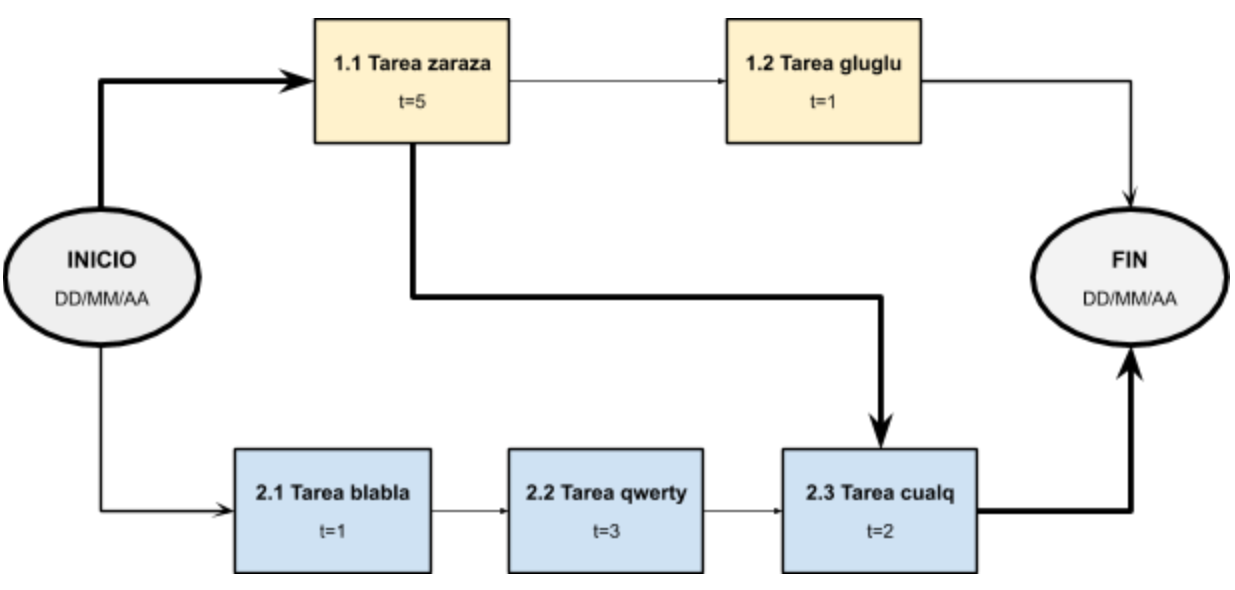
\includegraphics[width=.8\textwidth]{./Figuras/AoN.png}
\caption{Diagrama en \textit{Activity on Node}}
\label{fig:AoN}
\end{figure}

Indicar claramente en qué unidades están expresados los tiempos.
De ser necesario indicar los caminos semicríticos y analizar sus tiempos mediante un cuadro.
Es recomendable usar colores y un cuadro indicativo describiendo qué representa cada color, como se muestra en el siguiente ejemplo:



\section{8. Diagrama de Gantt}
\label{sec:gantt}

\begin{consigna}{red}
Utilizar el software Gantter for Google Drive o alguno similar para dibujar el diagrama de Gantt.

Existen muchos programas y recursos \textit{online} para hacer diagramas de gantt, entre las cuales destacamos:

\begin{itemize}
\item Planner
\item GanttProject
\item Trello + \textit{plugins}. En el siguiente link hay un tutorial oficial: \\ \url{https://blog.trello.com/es/diagrama-de-gantt-de-un-proyecto}
\item Creately, herramienta online colaborativa. \\\url{https://creately.com/diagram/example/ieb3p3ml/LaTeX}
\item Se puede hacer en latex con el paquete \textit{pgfgantt}\\ \url{http://ctan.dcc.uchile.cl/graphics/pgf/contrib/pgfgantt/pgfgantt.pdf}
\end{itemize}

Pegar acá una captura de pantalla del diagrama de Gantt, cuidando que la letra sea suficientemente grande como para ser legible. 
Si el diagrama queda demasiado ancho, se puede pegar primero la ``tabla'' del Gantt y luego pegar la parte del diagrama de barras del diagrama de Gantt.

Configurar el software para que en la parte de la tabla muestre los códigos del EDT (WBS).\\
Configurar el software para que al lado de cada barra muestre el nombre de cada tarea.\\
Revisar que la fecha de finalización coincida con lo indicado en el Acta Constitutiva.

En la figura \ref{fig:gantt}, se muestra un ejemplo de diagrama de gantt realizado con el paquete de \textit{pgfgantt}. En la plantilla pueden ver el código que lo genera y usarlo de base para construir el propio.

\begin{figure}[htbp]
\begin{center}
\begin{ganttchart}{1}{12}
  \gantttitle{2020}{12} \\
  \gantttitlelist{1,...,12}{1} \\
  \ganttgroup{Group 1}{1}{7} \\
  \ganttbar{Task 1}{1}{2} \\
  \ganttlinkedbar{Task 2}{3}{7} \ganttnewline
  \ganttmilestone{Milestone o hito}{7} \ganttnewline
  \ganttbar{Final Task}{8}{12}
  \ganttlink{elem2}{elem3}
  \ganttlink{elem3}{elem4}
\end{ganttchart}
\end{center}
\caption{Diagrama de gantt de ejemplo}
\label{fig:gantt}
\end{figure}

\end{consigna}

\section{9. Matriz de uso de recursos de materiales}
\label{sec:recursos}


\begin{table}
\label{tab:recursos}
\centering
\begin{tabularx}{\linewidth}{@{}|c|X|X|X|X|c|@{}}
\hline
\cellcolor[HTML]{C0C0C0} & \cellcolor[HTML]{C0C0C0} & \multicolumn{4}{c|}{\cellcolor[HTML]{C0C0C0}Recursos requeridos (horas)} \\ \cline{3-6} 
\multirow{-2}{*}{\cellcolor[HTML]{C0C0C0}\begin{tabular}[c]{@{}c@{}}Código\\ WBS\end{tabular}} & \multirow{-2}{*}{\cellcolor[HTML]{C0C0C0}\begin{tabular}[c]{@{}c@{}}Nombre \\ tarea\end{tabular}} & Material 1 & Material 2 & Material 3 & Material 4 \\ \hline
 &  &  &  &  &  \\ \hline
 &  &  &  &  &  \\ \hline
 &  &  &  &  &  \\ \hline
 &  &  &  &  &  \\ \hline
 &  &  &  &  &  \\ \hline
 &  &  &  &  &  \\ \hline
 &  &  &  &  &  \\ \hline
 &  &  &  &  &  \\ \hline 
 &  &  &  &  &  \\ \hline
 &  &  &  &  &  \\ \hline
 &  &  &  &  &  \\ \hline
 &  &  &  &  &  \\ \hline
 &  &  &  &  &  \\ \hline
 &  &  &  &  &  \\ \hline
 &  &  &  &  &  \\ \hline
 &  &  &  &  &  \\ \hline
 &  &  &  &  &  \\ \hline
 &  &  &  &  &  \\ \hline
 &  &  &  &  &  \\ \hline
 &  &  &  &  &  \\ \hline
 &  &  &  &  &  \\ \hline
 &  &  &  &  &  \\ \hline
 &  &  &  &  &  \\ \hline
 &  &  &  &  &  \\ \hline 
 &  &  &  &  &  \\ \hline
 &  &  &  &  &  \\ \hline
 &  &  &  &  &  \\ \hline
 &  &  &  &  &  \\ \hline

\end{tabularx}%
\end{table}


\section{10. Presupuesto detallado del proyecto}
\label{sec:presupuesto}

\begin{consigna}{red}
Si el proyecto es complejo entonces separarlo en partes:
\begin{itemize}
\item Un total global, indicando el subtotal acumulado por cada una de las áreas.
\item El desglose detallado del subtotal de cada una de las áreas.
\end{itemize}

IMPORTANTE: No olvidarse de considerar los COSTOS INDIRECTOS.

\end{consigna}

\begin{table}[htpb]
\centering
\begin{tabularx}{\linewidth}{@{}|X|c|r|r|@{}}
\hline
\rowcolor[HTML]{C0C0C0} 
\multicolumn{4}{|c|}{\cellcolor[HTML]{C0C0C0}COSTOS DIRECTOS} \\ \hline
\rowcolor[HTML]{C0C0C0} 
Descripción &
  \multicolumn{1}{c|}{\cellcolor[HTML]{C0C0C0}Cantidad} &
  \multicolumn{1}{c|}{\cellcolor[HTML]{C0C0C0}Valor unitario} &
  \multicolumn{1}{c|}{\cellcolor[HTML]{C0C0C0}Valor total} \\ \hline
 &
  \multicolumn{1}{c|}{} &
  \multicolumn{1}{c|}{} &
  \multicolumn{1}{c|}{} \\ \hline
 &
  \multicolumn{1}{c|}{} &
  \multicolumn{1}{c|}{} &
  \multicolumn{1}{c|}{} \\ \hline
\multicolumn{1}{|l|}{} &
   &
   &
   \\ \hline
\multicolumn{1}{|l|}{} &
   &
   &
   \\ \hline
\multicolumn{3}{|c|}{SUBTOTAL} &
  \multicolumn{1}{c|}{} \\ \hline
\rowcolor[HTML]{C0C0C0} 
\multicolumn{4}{|c|}{\cellcolor[HTML]{C0C0C0}COSTOS INDIRECTOS} \\ \hline
\rowcolor[HTML]{C0C0C0} 
Descripción &
  \multicolumn{1}{c|}{\cellcolor[HTML]{C0C0C0}Cantidad} &
  \multicolumn{1}{c|}{\cellcolor[HTML]{C0C0C0}Valor unitario} &
  \multicolumn{1}{c|}{\cellcolor[HTML]{C0C0C0}Valor total} \\ \hline
\multicolumn{1}{|l|}{} &
   &
   &
   \\ \hline
\multicolumn{1}{|l|}{} &
   &
   &
   \\ \hline
\multicolumn{1}{|l|}{} &
   &
   &
   \\ \hline
\multicolumn{3}{|c|}{SUBTOTAL} &
  \multicolumn{1}{c|}{} \\ \hline
\rowcolor[HTML]{C0C0C0}
\multicolumn{3}{|c|}{TOTAL} &
   \\ \hline
\end{tabularx}%
\end{table}


\section{11. Matriz de asignación de responsabilidades}
\label{sec:responsabilidades}
\begin{consigna}{red}
Establecer la matriz de asignación de responsabilidades y el manejo de la autoridad completando la siguiente tabla:

\begin{table}[htpb]
\centering
\resizebox{\textwidth}{!}{%
\begin{tabular}{|c|c|c|c|c|c|}
\hline
\rowcolor[HTML]{C0C0C0} 
\cellcolor[HTML]{C0C0C0} &
  \cellcolor[HTML]{C0C0C0} &
  \multicolumn{4}{c|}{\cellcolor[HTML]{C0C0C0}Listar todos los nombres y roles del proyecto} \\ \cline{3-6} 
\rowcolor[HTML]{C0C0C0} 
\cellcolor[HTML]{C0C0C0} &
  \cellcolor[HTML]{C0C0C0} &
  Responsable &
  Orientador &
  Equipo &
  Cliente \\ \cline{3-6} 
\rowcolor[HTML]{C0C0C0} 
\multirow{-3}{*}{\cellcolor[HTML]{C0C0C0}\begin{tabular}[c]{@{}c@{}}Código\\ WBS\end{tabular}} &
  \multirow{-3}{*}{\cellcolor[HTML]{C0C0C0}Nombre de la tarea} &
  \authorname &
  \supname &
  Nombre de alguien &
  \clientename \\ \hline
 &  &  &  &  &  \\ \hline
 &  &  &  &  &  \\ \hline
 &  &  &  &  &  \\ \hline
\end{tabular}%
}
\end{table}

{\footnotesize
Referencias:
\begin{itemize}
	\item P = Responsabilidad Primaria
	\item S = Responsabilidad Secundaria
	\item A = Aprobación
	\item I = Informado
	\item C = Consultado
\end{itemize}
} %footnotesize

Una de las columnas debe ser para el Director, ya que se supone que participará en el proyecto.
A su vez se debe cuidar que no queden muchas tareas seguidas sin ``A'' o ``I''.

Importante: es redundante poner ``I/A'' o ``I/C'', porque para aprobarlo o responder consultas primero la persona debe ser informada.

\end{consigna}

\section{12. Gestión de riesgos}
\label{sec:riesgos}

\begin{consigna}{red}
a) Identificación de los riesgos (al menos cinco) y estimación de sus consecuencias:
 
Riesgo 1: detallar el riesgo (riesgo es algo que si ocurre altera los planes previstos)
\begin{itemize}
\item Severidad (S): mientras más severo, más alto es el número (usar números del 1 al 10).\\
Justificar el motivo por el cual se asigna determinado número de severidad (S).
\item Probabilidad de ocurrencia (O): mientras más probable, más alto es el número (usar del 1 al 10).\\
Justificar el motivo por el cual se asigna determinado número de (O). 
\end{itemize}   

Riesgo 2:
\begin{itemize}
\item Severidad (S): 
\item Ocurrencia (O):
\end{itemize}

Riesgo 3:
\begin{itemize}
\item Severidad (S): 
\item Ocurrencia (O):
\end{itemize}


b) Tabla de gestión de riesgos:      (El RPN se calcula como RPN=SxO)

\begin{table}[htpb]
\centering
\begin{tabularx}{\linewidth}{@{}|X|c|c|c|c|c|c|@{}}
\hline
\rowcolor[HTML]{C0C0C0} 
Riesgo & S & O & RPN & S* & O* & RPN* \\ \hline
       &   &   &     &    &    &      \\ \hline
       &   &   &     &    &    &      \\ \hline
       &   &   &     &    &    &      \\ \hline
       &   &   &     &    &    &      \\ \hline
       &   &   &     &    &    &      \\ \hline
\end{tabularx}%
\end{table}

Criterio adoptado: 
Se tomarán medidas de mitigación en los riesgos cuyos números de RPN sean mayores a...

Nota: los valores marcados con (*) en la tabla corresponden luego de haber aplicado la mitigación.

c) Plan de mitigación de los riesgos que originalmente excedían el RPN máximo establecido:
 
Riesgo 1: plan de mitigación (si por el RPN fuera necesario elaborar un plan de mitigación).
  Nueva asignación de S y O, con su respectiva justificación:
  - Severidad (S): mientras más severo, más alto es el número (usar números del 1 al 10).
          Justificar el motivo por el cual se asigna determinado número de severidad (S).
  - Probabilidad de ocurrencia (O): mientras más probable, más alto es el número (usar del 1 al 10).
          Justificar el motivo por el cual se asigna determinado número de (O).

Riesgo 2: plan de mitigación (si por el RPN fuera necesario elaborar un plan de mitigación).
 
Riesgo 3: plan de mitigación (si por el RPN fuera necesario elaborar un plan de mitigación).

\end{consigna}


\section{13. Gestión de la calidad}
\label{sec:calidad}

\begin{consigna}{red}
Para cada uno de los requerimientos del proyecto indique:
\begin{itemize} 
\item Req \#1: copiar acá el requerimiento.

Verificación y validación:

\begin{itemize}
\item Verificación para confirmar si se cumplió con lo requerido antes de mostrar el sistema al cliente. Detallar 
\item Validación con el cliente para confirmar que está de acuerdo en que se cumplió con lo requerido. Detallar  
\end{itemize}

\end{itemize}

Tener en cuenta que en este contexto se pueden mencionar simulaciones, cálculos, revisión de hojas de datos, consulta con expertos, mediciones, etc.

\end{consigna}

\section{14. Comunicación del proyecto}
\label{sec:comunicaciones}

El plan de comunicación del proyecto es el siguiente:

\begin{table}[htpb]
\centering
\begin{tabularx}{\linewidth}{@{}|X|C{2.4cm}|C{3cm}|C{1.8cm}|C{2cm}|C{2.1cm}|@{}}
\hline
\rowcolor[HTML]{C0C0C0} 
\multicolumn{6}{|c|}{\cellcolor[HTML]{C0C0C0}PLAN DE COMUNICACIÓN DEL PROYECTO}           \\ \hline
\rowcolor[HTML]{C0C0C0} 
¿Qué comunicar? & Audiencia & Propósito & Frecuencia & Método de comunicac. & Responsable \\ \hline
                &           &           &            &                      &             \\ \hline
                &           &           &            &                      &             \\ \hline
                &           &           &            &                      &             \\ \hline
                &           &           &            &                      &             \\ \hline
                &           &           &            &                      &             \\ \hline
\end{tabularx}
\end{table}

\section{15. Gestión de compras}
\label{sec:compras}

\begin{consigna}{red}
En caso de tener que comprar elementos o contratar servicios:
a) Explique con qué criterios elegiría a un proveedor.
b) Redacte el Statement of Work correspondiente.
\end{consigna}

\section{16. Seguimiento y control}
\label{sec:seguimiento}

\begin{consigna}{red}
Para cada tarea del proyecto establecer la frecuencia y los indicadores con los se seguirá su avance y quién será el responsable de hacer dicho seguimiento y a quién debe comunicarse la situación (en concordancia con el Plan de Comunicación del proyecto).

El indicador de avance tiene que ser algo medible, mejor incluso si se puede medir en \% de avance. Por ejemplo,se pueden indicar en esta columna cosas como ``cantidad de conexiones ruteadeas'' o ``cantidad de funciones implementadas'', pero no algo genérico y ambiguo como ``\%'', porque el lector no sabe porcentaje de qué cosa.

\end{consigna}

\begin{longtable}{|m{1cm}|m{3.5cm}|m{2.2cm}|m{2cm}|m{3cm}|m{1.5cm}|}
\hline
\rowcolor[HTML]{C0C0C0} 
\multicolumn{6}{|c|}{\cellcolor[HTML]{C0C0C0}SEGUIMIENTO DE AVANCE}                                                                       \\ \hline
\rowcolor[HTML]{C0C0C0} 
Tarea del WBS 			& Indicador de avance & Frecuencia de reporte & Resp. de seguimiento & Persona a ser informada & Método de comunic. \\ \hline
\endfirsthead

\hline
\rowcolor[HTML]{C0C0C0} 
\multicolumn{6}{c}{\cellcolor[HTML]{C0C0C0}SEGUIMIENTO DE AVANCE}                                                                       \\ \hline
\rowcolor[HTML]{C0C0C0} 
Tarea del WBS 			& Indicador de avance & Frecuencia de reporte & Resp. de seguimiento & Persona a ser informada & Método de comunic. \\ \hline
\endhead

\multicolumn{6}{c}{Continúa}
\endfoot

\endlastfoot

1.1	& Fecha de inicio  & Única vez al comienzo & \authorname & \clientename, \supname & email \\ \hline
2.1	& Avance de las subtareas  & Mensual mientras dure la tarea & \authorname & \clientename, \supname & email \\ \hline

\end{longtable}

\begin{table}[!htpb]
\centering
%\begin{tabularx}{\linewidth}{@{}|X|X|X|X|X|X|@{}}
\begin{tabularx}{\linewidth}{@{}|X|C{2.5cm}|C{3cm}|C{2cm}|C{2cm}|C{2.5cm}|@{}}
\hline
\rowcolor[HTML]{C0C0C0} 
\multicolumn{6}{|c|}{\cellcolor[HTML]{C0C0C0}SEGUIMIENTO DE AVANCE}                                                                       \\ \hline
\rowcolor[HTML]{C0C0C0} 
Tarea del WBS & Indicador de avance & Frecuencia de reporte & Resp. de seguimiento & Persona a ser informada & Método de comunic. \\ \hline
 &  &  &  &  &  \\ \hline
 &  &  &  &  &  \\ \hline
 &  &  &  &  &  \\ \hline
 &  &  &  &  &  \\ \hline
 &  &  &  &  &  \\ \hline
\end{tabularx}%
%}
\end{table}

\section{17. Procesos de cierre}    
\label{sec:cierre}

\begin{consigna}{red}
Establecer las pautas de trabajo para realizar una reunión final de evaluación del proyecto, tal que contemple las siguientes actividades:

\begin{itemize}
\item Pautas de trabajo que se seguirán para analizar si se respetó el Plan de Proyecto original:
 - Indicar quién se ocupará de hacer esto y cuál será el procedimiento a aplicar. 
\item Identificación de las técnicas y procedimientos útiles e inútiles que se utilizaron, y los problemas que surgieron y cómo se solucionaron:
 - Indicar quién se ocupará de hacer esto y cuál será el procedimiento para dejar registro.
\item Indicar quién organizará el acto de agradecimiento a todos los interesados, y en especial al equipo de trabajo y colaboradores:
  - Indicar esto y quién financiará los gastos correspondientes.
\end{itemize}

\end{consigna}


\end{document}
